\chapter{結論}
\label{chap:conclusion}

\section{満足性評価のための指標}

\subsection{提案}

\subsection{妥当性の検討}

\section{時系列UX評価システム}

\subsection{提案}

\subsection{妥当性の検討}

\section{今後の課題}

\subsection{満足性評価指標}

\subsection{時系列UX評価システム}

\subsection{統合的なシステムとしての展望}

\begin{figure}[htbp]
  \begin{minipage}{0.5\hsize}
    \begin{center}
       \includegraphics[width=70mm]{img/design_record_1}
    \end{center}
    \caption{測定画面のプロトタイプ(アプリ用)}
    \label{fig:futurework1}
  \end{minipage}
    \begin{minipage}{0.5\hsize}
    \begin{center}
       \includegraphics[width=70mm]{img/design_record_2}
    \end{center}
    \caption{測定画面のプロトタイプ(VR用)}
    \label{fig:futurework2}
  \end{minipage}
\end{figure}


\begin{figure}[htbp]
  \begin{minipage}{\hsize}
    \begin{center}
       \includegraphics[width=100mm]{img/design_analyze}
    \end{center}
    \caption{分析画面のプロトタイプ}
    \label{fig:futurework3}
  \end{minipage}
\end{figure}

\begin{figure}[htbp]
  \begin{minipage}{\hsize}
    \begin{center}
       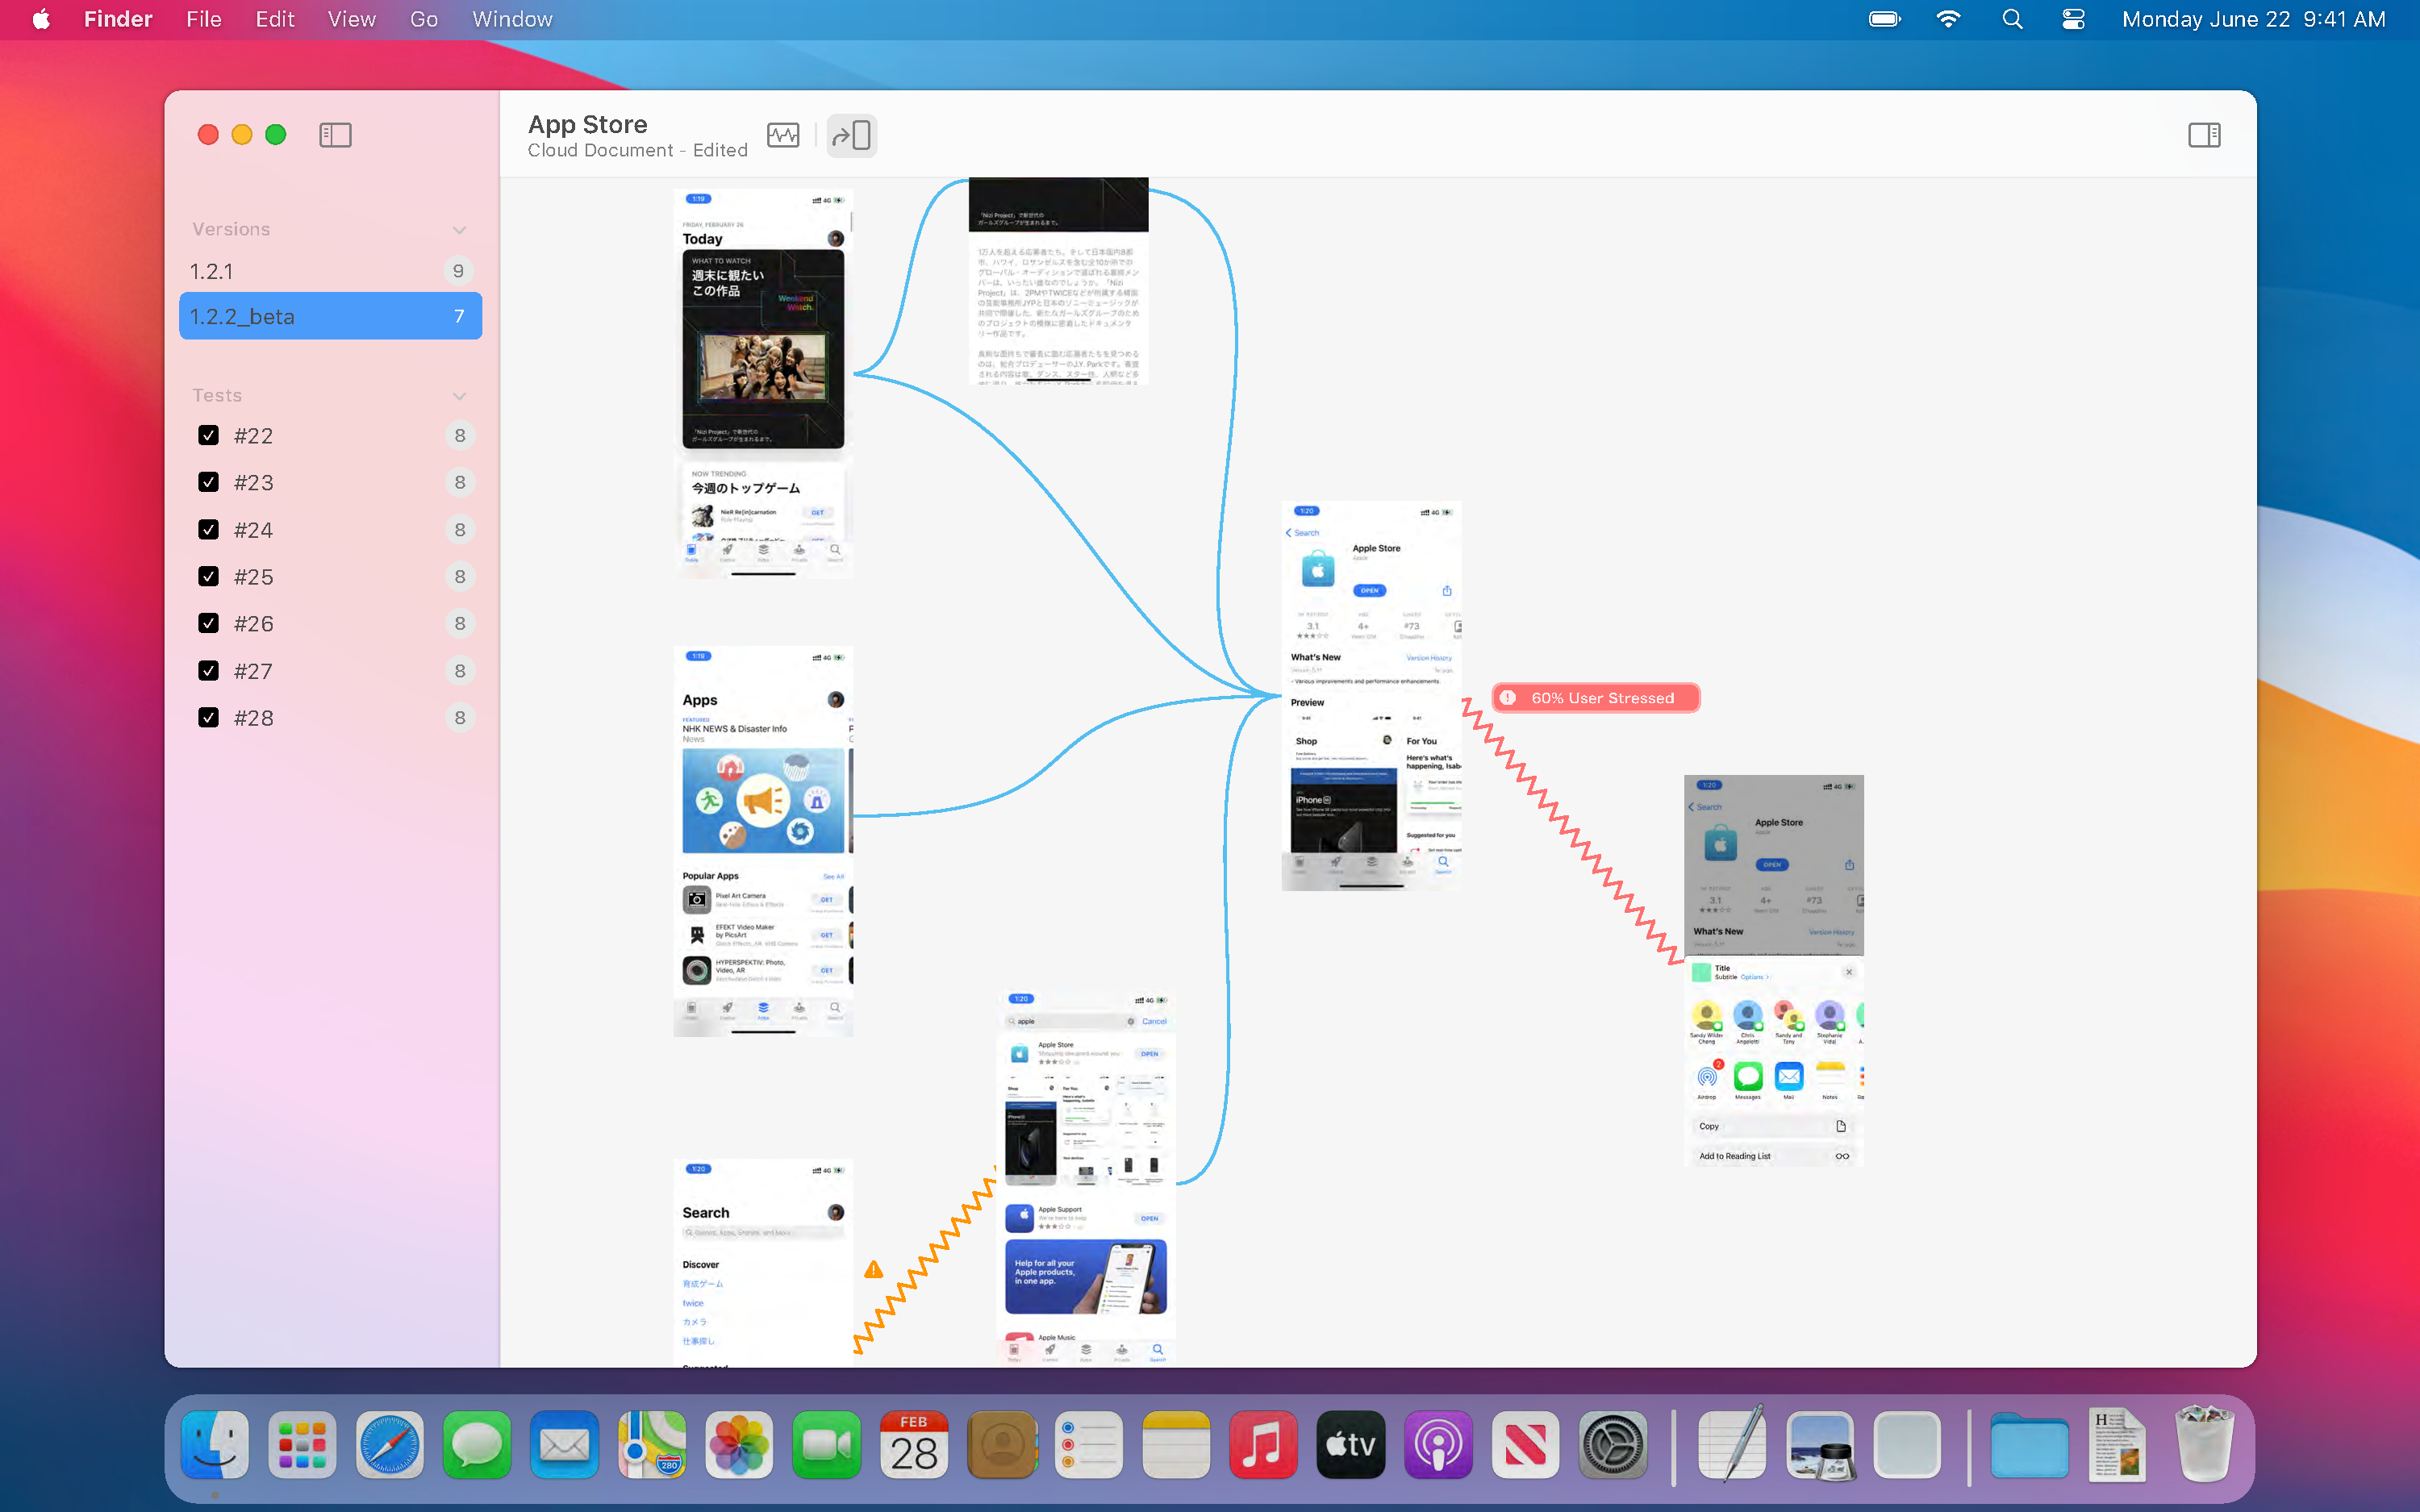
\includegraphics[width=100mm]{img/design_storyboard}
    \end{center}
    \caption{画面遷移図での可視化画面のプロトタイプ}
    \label{fig:futurework4}
  \end{minipage}
\end{figure}
